\clearpage
\subsection{Getting started with MOSL}
\texHeader
\hypertarget{static:starting tex}{}

\begin{itemize}

\item[$\blacktriangleright$] \hypertarget{static tex}{Begin a} new metamodel project from eclipse by navigating to the \texttt{New Metamodel} button on the
toolbar. In the dialog that appears, enter \texttt{LeitnersLearningBox} as the project name, and select \texttt{Textual (MOSL)}  (Fig.~\ref{fig:new_project}).

\begin{figure}[htbp]
	\centering
  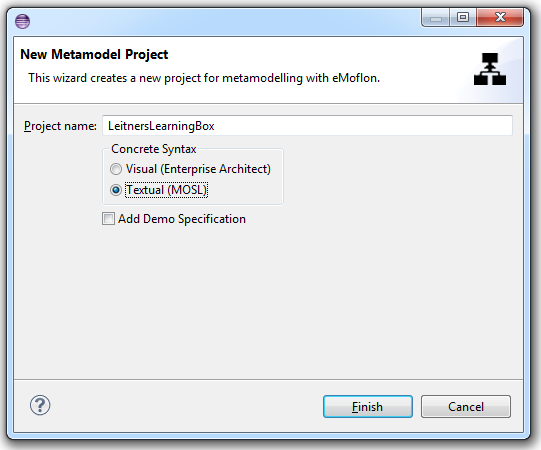
\includegraphics[width=0.6\textwidth]{eclipse_newMetamodelTextPlain}
	\caption{Create a new concrete metamodeling project}
	\label{fig:new_project}
\end{figure}

\item[$\blacktriangleright$] Expand the project as deep as it goes. Your Package explorer may look different than ours (Fig.~\ref{fig:expanded_folders})
depending on whether or not you completed the Demo in Part I. In an effort to keep things clear as possible, we have removed them from our workspaces, but
recommend keeping them for future reference.

\begin{figure}[htbp]
	\centering
  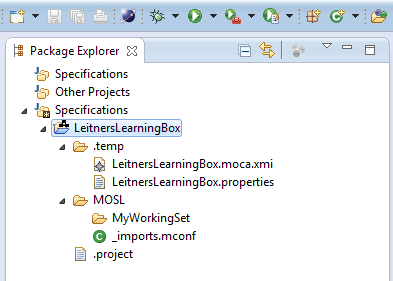
\includegraphics[width=0.5\textwidth]{eclipse_foldersExpanded}
	\caption{Expanded project files}
	\label{fig:expanded_folders}
\end{figure} 

\clearpage
\item[$\blacktriangleright$] You can see two folders, \texttt{.temp}, and \texttt{MOSL}, and one subfolder, \texttt{MyWorkingSet}, inside the
\texttt{Specifications} node\footnote{for detailed review on the explorer structre, look over Part I}. We're most insterested in \texttt{MyWorkingSet}, which
stores the collection of files and  \emph{unifies} everything we need for Leitner's Box.

\item[$\blacktriangleright$] Right click on your current workspace folder, \texttt{MyWorkingSet}, and create a new subfolder. Name it
\texttt{LearningBoxLanguage}. This is now the container for all your modelling files!


\item[$\blacktriangleright$] That's all you needed to do to start a new project! (Some sort of finalizing remark\ldots)

\fancyfoot[R]{$\triangleright$ \hyperlink{static:classes tex}{Next}}

\end{itemize}
